\subsection{Tecnología}

Siempre que sea aplicable, la inspiración se extrae de la analogía con las Capas de Negocio y Aplicación. La Capa de Tecnología se utiliza típicamente para modelar la arquitectura tecnológica de la empresa, definida por el marco TOGAF como: "la estructura e interacción de los servicios de la plataforma, y los componentes tecnológicos lógicos y físicos".

\newpage
\subsubsection{Elementos de la Estructura}
\begin{longtable}{|c|c|c|}
	%\{table}
	%	\subsection{Capa Tecnologica}
	%\begin{center}
	%\begin{tabular}{| l | c | l |}
	% estructura activa
	\hline
	Concepto & Descripción & Representación \\ \hline
	Nodo
	& 
	\begin{tabular}{p{8cm}p{3cm}}
		Recurso sobre el cual se almacenan los artefactos.
		Es un recurso que se considera fisico y computacional al mismo tiempo, el cual se aloja, manipula e interactua con los demas recursos fisicos o computacionales. Elementos de estructura activa que 
		ejecutan, almacenan y Procesan objetos de tecnología como artefactos. Se conectan por medio de las rutas. El nombre de un nodo debe ser preferiblemente un sustantivo. Un nodo puede contener subnodos. Los artefactos desplegados en un nodo pueden dibujarse dentro del nodo o conectarse a él con un Relación de asignación.
	\end{tabular}
	& 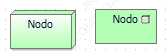
\includegraphics[width=0.2\linewidth, height=0.05\textheight]{imgs/conceptos/tecnologica/nodo}
	\\
	\hline
	Dispositivo
	&
	\begin{tabular}{p{8cm}p{3cm}} 
		Recurso de hardware que almacena o despliega para su ejecucion. 
		Es un dispositvo de recurso TI físico, en los cuales se almacena el software del sistema y los artefactos desplegado para su ejecución.
		La forma especializada de un nodo es un dispositivo el cual representa un recurso de TI físico con procesamiento y capacidad.
		Por lo general es utilizado en el modelamiento de sistemas de hardware tales como mainframes, PC o enrutadores.
		Puede ser compuesto, es decir con subdispositivos. El nombre debe ser preferiblemente un sustantivo, para su distincion se puede usar 
		iconos.
		
	\end{tabular}
	& 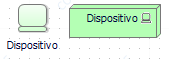
\includegraphics[width=0.2\linewidth, height=0.05\textheight]{imgs/conceptos/tecnologica/dispositivo}
	\\
	\hline
	
	\begin{tabular}{p{2cm}p{3cm}}
		Software de sistema
	\end{tabular}
	&
	\begin{tabular}{p{8cm}p{3cm}} 
		Entorno de software para componentes y objetos que se iplementan en forma de artefactos.
		El software del sistema proporciona un entorno para almacenar, ejecutar y usar software implementado en el.
		Es la especializacion de un nodo usado para modelar el entonrno de software en artefactos funcionales, tambien se puede utilizar
		para representaciones como middleware de comunicacion.
		se puede asignar un software del sistema a otro, con el fin de crear capas de software que se ejecutan una encima de otra. 
		El nombre del sistema debe ser un sustantivo que se refiera a tipo de ejecucion.
		
	\end{tabular}
	& 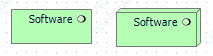
\includegraphics[width=0.2\linewidth, height=0.05\textheight]{imgs/conceptos/tecnologica/software}
	\\
	\hline
	
	Colaboracion
	&
	\begin{tabular}{p{8cm}p{3cm}} 
		Es un agregado de dos o mas nodos que trabajan juntos para realizar un comportamiento tecnologico colectivo, la misma especifica que nodos
		cooperan para realizar alguna tarea, la colaboración tecnológica puede estar compuesta por interfaces tecnológicas y una interfaz tecnologica puede servir para una colaboracion tencnologica. El nombre de una colaboracion tecnologica debe ser un sustantivo.
		
	\end{tabular}
	& 
\includegraphics[width=0.2\linewidth, height=0.05\textheight]{imgs/conceptos/tecnologica/colaboracion}
	\\			
	\hline
	\begin{tabular}{p{2cm}p{3cm}}
		Interfaz de infraestructura
	\end{tabular}
	&
	\begin{tabular}{p{8cm}p{3cm}} 
		Punto de acceso donde se los servicios pueden ser utilizados.
		Es la representacion de un punto de acceso desde el cual los servicios de un nodo pueden ser accesibles.
		Especifica como otros usuarios acceden a los servicios de un nodo, deja un servicio tecnologico al medio ambiente y asi mismo puede exponerse
		a traves de diferentes interfaces.
		Una interfaz tecnologica puede ser parte de un nodo a traves de la composicion, lo cual quiere decir que son proporcionadas por este y pueden servir 
		a otros nodos.
		El nombre de una interfaz tecnologica debe ser preferiblemente un sustantivo
		
	\end{tabular}
	& 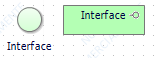
\includegraphics[width=0.2\linewidth, height=0.05\textheight]{imgs/conceptos/tecnologica/interfaceTecnologia}
	\\
	\hline
	
	\begin{tabular}{p{2cm}p{3cm}}
		Ruta de comunicacion 
	\end{tabular}
	&
	\begin{tabular}{p{8cm}p{3cm}} 
		Es la representacion del enlace entre dos o mas nodos, a traves de la cual estos intercambian datos o material, se utiliza una ruta para modelar
		las relaciones logicas de comunicacion entre nodos. Una ruta se realiza mediante una o más redes un camino puede ser agregando por nodos.
		
	\end{tabular} 
	& 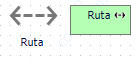
\includegraphics[width=0.2\linewidth, height=0.05\textheight]{imgs/conceptos/tecnologica/ruta}
	\\
	\hline
	
	Red
	&
	\begin{tabular}{p{8cm}p{3cm}}
		Medio de comunicacion entre varios dispositivos. 
		Una red de comunicación representa un conjunto de estructuras que conecta sistemas informáticos u otros dispositivos electrónicos para 
		transmisión, enrutamiento y recepción de datos o comunicaciones basadas en datos como voz y video. Es la representacion de la insfraestructura de la comunicacion fisica entre sistemas. Una red tiene propiedades como ancho de banda y latencia, esta es realizada por una o mas rutas.
		Puede constar de subredes y agregar dispositivos y sistemas de software.
		
	\end{tabular}	
	& 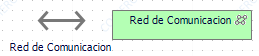
\includegraphics[width=0.2\linewidth, height=0.05\textheight]{imgs/conceptos/tecnologica/redComunicacion}
	\\
	\hline
	
	% Comportamiento			
	\begin{tabular}{p{2cm}p{3cm}}
		Funcion infraestructura 
	\end{tabular}
	&
	\begin{tabular}{p{8cm}p{3cm}}
		Comportamiento basico, agrupado de los extraidos de un nodo 
		Una función tecnológica representa un conjunto de comportamientos tecnológicos que puede realizar un nodo.Una función tecnológica describe el comportamiento interno de un nodo; para el usuario de un nodo que realiza una función tecnológica. Si su comportamiento se expone externamente,esto se hace a través de uno o más servicios tecnológicos. El nombre de una función tecnológica debe ser preferiblemente una terminación de verbocon "ing"
	\end{tabular}
	& 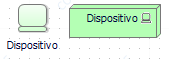
\includegraphics[width=0.2\linewidth, height=0.05\textheight]{imgs/conceptos/tecnologica/dispositivo}
	\\
	\hline
	
	\begin{tabular}{p{2cm}p{3cm}}
		Proceso tecnologico
	\end{tabular}
	&
	\begin{tabular}{p{8cm}p{3cm}} 
		Un proceso tecnológico representa una secuencia de comportamientos tecnológicos que logra una salida. Un proceso tecnológico describe el comportamiento interno de un nodo; para el usuario de ese nodo, este proceso es invisible. Si su comportamiento se expone externamente, esto se hace a través de uno o más servicios tecnológicos. Puede utilizar objetos tecnológicos como entrada y utilizar o transformar estos para producir otros objetos tecnológicos como salida.
	\end{tabular}
	& 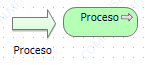
\includegraphics[width=0.2\linewidth, height=0.05\textheight]{imgs/conceptos/tecnologica/procesoTecnologia}
	\\
	\hline
	
	Interaccion 
	&
	\begin{tabular}{p{8cm}p{3cm}} 
		Una interacción tecnológica representa una unidad de comportamiento tecnológico colectivo realizado por dos o más nodos. Una interacción tecnológica describe el comportamiento colectivo que realizan los nodos que participan en una colaboración tecnológica. Esto puede incluir, por ejemplo, la comunicaciónpatrón entre estos componentes. Una interacción tecnológica también puede especificar externamente comportamiento visible necesario para realizar un servicio tecnológico. Una la interacción puede realizar un servicio tecnológico.
	\end{tabular}
	& 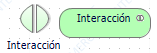
\includegraphics[width=0.2\linewidth, height=0.05\textheight]{imgs/conceptos/tecnologica/InteraccionTecnologia}
	\\
	\hline
	
	Evento 
	&
	\begin{tabular}{p{8cm}p{3cm}} 
		Un evento tecnológico es un elemento de comportamiento tecnológico que denota un cambio de estado. A diferencia de los procesos, funciones e interacciones, un evento es instantáneo: no tienen duración. Puede tener un atributo de tiempo que denota el momento o momentos en los que ocurre el evento. Puede ser desencadenado por una función, y puede estar compuesto por otros eventos tecnológicos. El nombre de un evento tecnológico debe ser preferiblemente un verbo en tiempo perfecto 
	\end{tabular}
	& 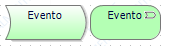
\includegraphics[width=0.2\linewidth, height=0.05\textheight]{imgs/conceptos/tecnologica/eventoTecnologia}
	\\
	\hline
	
	\begin{tabular}{p{2cm}p{3cm}}
		infraestructura de servicio  
	\end{tabular}
	&
	\begin{tabular}{p{8cm}p{3cm}} 
		Unidad funcional visible de varios nodos por medio de interfaces.
		Un servicio de tecnología representa un comportamiento tecnológico expuesto explícitamente definido.Un servicio tecnológico expone la funcionalidad de un nodo a su entorno. Esta funcionalidad esse accede a través de una o más interfaces tecnológicas. Puede requerir, usar y producir artefactos.Los servicios tecnológicos típicos pueden incluir, por ejemplo, mensajería, almacenamiento, nombres ydirectorio de Servicios. Puede acceder a artefactos; por ejemplo, un archivo que contiene un mensaje. Un servicio de tecnología puede acceder a artefactos. Una tecnología el servicio puede consistir en sub-servicios.El nombre de un servicio de tecnología debería ser preferiblemente un verbo que termine con “ia”; p.ej,"mensajería". Además, se puede utilizar un nombre que contenga explícitamente la palabra "servicio".
	\end{tabular} 
	& 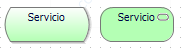
\includegraphics[width=0.2\linewidth, height=0.05\textheight]{imgs/conceptos/tecnologica/servicioTecnologia}
	\\
	\hline
	
	% estructura pasiva
	
	\begin{tabular}{p{2cm}p{3cm}}
		Objeto tecnologico
	\end{tabular}
	&
	\begin{tabular}{p{8cm}p{3cm}} 
		Un objeto tecnológico representa un elemento pasivo que es utilizado o producido por el comportamiento.Los objetos tecnológicos representan los objetos "físicos" manipulados por la infraestructura de una empresa, puede incluir artefactos (por ejemplo, archivos) como material físico.Se puede acceder a los objetos tecnológicos mediante el comportamiento tecnológico (funciones, procesos, interacciones,eventos y servicios). El nombre de un objeto tecnológico debe ser preferiblemente un sustantivo
	\end{tabular}
	& 
\includegraphics[width=0.2\linewidth, height=0.05\textheight]{imgs/conceptos/tecnologica/Ud}
	\\
	\hline
	
	Artefacto
	&
	\begin{tabular}{p{8cm}p{3cm}} 
		Puede ser una pieza fisica de datos que se genera o utiliza en el proceso de desarrollo.
		Representa un dato que se utiliza o produce en un proceso de desarrollo de software, de igual manera representa un elemiento tangible en el mundo de las TI, normalmente es utlizado para modelar productos como archivos fuente, ejecutables, scripts, tablas de bases de datos, mensajes, etc.
		Mediantes uno o mas artefactos se pueden realizar componentes de software por lo cual las dos formas tipicas de utilizar el elemento son como un componente de ejecucion o un archivo de datos. Puede constar de sub-artefactos y el nombre debe ser preferiblemente el del archivo que representa.
		
	\end{tabular}
	& 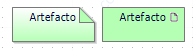
\includegraphics[width=0.2\linewidth, height=0.05\textheight]{imgs/conceptos/tecnologica/artefacto}
	\\
	
	\hline
	%\end{tabular}
			\caption{Conceptos Tecnología}
	%		\label{tab:concepts}
	%\end{center}
	%\end{table}
\end{longtable}